\begin{figure}
  \centering
  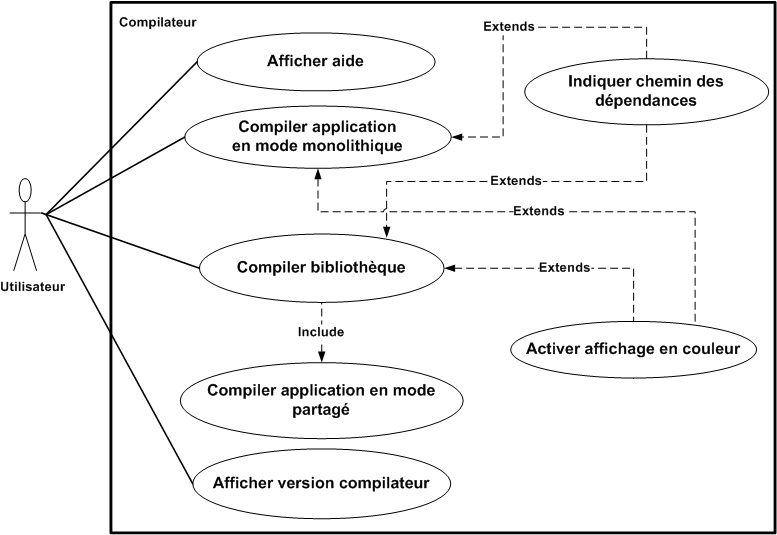
\includegraphics[scale=0.8]{../res/stb/vs_finale_usecase.jpg}
  \caption{\textbf{Cas d'utilisations du compilateur kawa.}}
\end{figure}

%Cas d'utilisation
\subsection{Cas d'utilisation EF\_1}
\fiche
{Afficher l'aide}                    % Nom du cas d'utilisation
{Utilisateur du compilateur}                               % Acteurs concernés
{                                                % Description
  le compilateur affiche 
   la liste des options du compilateur sur la sortie standard à travers une ligne de commande.
}
{
  L'odre de priorité entre le commutateur de help (-h ou --help) et le commutateur de version (-v ou --version) est définit par la première occurrence de l'un des deux commutateur i-e si nous avons un \textbf {-h} avant un \textbf {-v}, le compilateur annule tout le reste et affiche le help 
}                                                % Préconditions
{Commutateur de ligne de commande :kawac -h ou --help}                             % Evénements déclenchants
{Fin du programme.}                       % Conditions d'arrêt
% {0.6}{../res/stb/usecase2_flot_event.png}      % Diagramme
{} % acteur(s)
{} % system
{} % flot exceptionsb
 % fin usecase EF_1

\subsection{Cas d'utilisation EF\_2}
\fiche
{Compiler une application en mode monolithique}                    % Nom du cas d'utilisation
{Utilisateur du compilateur}                               % Acteurs concernés
{                                                % Description
  L'utilisateur introduit un ensemble de classes
  kawa afin de les précompiler et de générer le tout dans un seul exécutable.
}
{
	Ensemble de fichiers sources contenant obligatoirement la méthode main qui constitue le point d'entrée de l'application, les sources fournies par l'utilisateur doivent respecter la syntaxe du langage kawa.
	La non présence des deux commutateurs (-h ou --help) et (-v ou --version) dans la ligne de commande permettant la compilation est obligatoire.
}                                                % Préconditions
{
Afin de déclencher le processus de compilation en mode monolithique, il faut fournir un fichier source contenant obligatoirement la méthode main, ainsi que l'utilisateur doit préciser le mode de compilation qui est le mode monolithique grâce au commutateur de ligne de commande :kawac -m filessources.}    % Evénements déclenchants
{
	Fin de la compilation sans erreurs dans ces différentes étapes d'analyses, ainsi que la production d’un seul exécutable qui ne dépend d'aucune bibliothèque externe ni de bibliothèques dynamiques.  
}  % Conditions d'arrêt
%{0.6}{../res/stb/usecase2_flot_event.png} 		 % Diagramme
{                                                % Flots d'exceptions
  
}
{} % system
{La compilation peut être interrompue pour divers raisons, on cite comme exemple la non fourniture de la méthode \textbf {main} dans les fichiers sources, sachant qu'elle est obligatoire pour le processus de compilation dans ce mode, elle peut être arrêtée aussi à travers les erreurs rencontrés dans les différentes étapes d'analyses du code source  tels que l'analyse lexicale, syntaxique ou bien l'analyse sémantique, le compilateur doit renvoyer des messages d'erreurs pour l'utilisateur afin qu'il les corrige dans le but d'accomplir la compilation du programme et de générer son exécutable.  } % flot exceptions
% Fin de la fiche du cas d'utilisation 1.


%Cas d'utilisation 2
\subsection{Cas d'utilisation EF\_3}
\fiche
{Compiler une application en mode partagé}                    % Nom du cas d'utilisation
{Utilisateur du compilateur}                               % Acteurs concernés
{                                                % Description
  L’utilisateur introduit un ensemble de sources kawa
 qui peuvent appelés des bibliothèques externes, le compilateur doit être capable de chercher les bibliothèques pour les utiliser ou bien  de les recompiler si nécessaire.la différence entre ce mode et le mode monolithique est que Le fichier exécutable et la bibliothèque sont indépendants avant le lancement de l’application, et peuvent être maintenus séparément à l'encontre du mode monolithique qui génère un seul exécutable regroupant le tout.Pour les bibliothèques partagées l'édition des liens se fait à l’exécution (au moment du lancement du programme) au contraire des bibliothèques statiques où l'édition des liens se fait dans la phase de compilation. 
}
{
	Ensemble de fichiers source respectant la syntaxe du langage kawa qui peuvent utiliser des bibliothèques partagées.La non présence des deux commutateurs (-h ou --help) et (-v ou --version) dans la ligne de commande permettant la compilation est obligatoire, ainsi que l'absence de commutateur indiqant qu'on est dans le mode monolithique. 
	
}                                                % Préconditions
{Afin de déclencher le processus de compilation en mode partagé, l'utilisateur introduit ces fichiers sources qui peuvent faire des appels vers des bibliothèques partagées, la présence de la méthode main est obligatoire pour compiler l'application ,sachant qu'il peut compiler en parallèle d'autres bibliothèque même si elle ne sont pas en relation avec l'application à compiler, ainsi  l'utilisateur doit préciser le mode de compilation qui est le mode partagé grâce au commutateur de ligne de commande :kawac filessources [options].}  % Evénements déclenchants
{
Fin de la compilation sans erreurs dans ces différentes étapes d'analyses, Le compilateur produit un exécutable léger par rapport au mode monolithique car le fichier exécutable ne contiendra pas le code de la librairie à laquelle il est lié, il est indépendant de la bibliothèque jusqu'à le lancement de l'application où il y' aura une édition des liens et le code contenu dans la librairie sera chargé.} % Conditions d'arrêt
%{0.6}{../res/stb/usecase2_flot_event.png} 		 % Diagramme
{                                                % Flots d'exceptions
  
}{} % system
{La compilation peut être interrompue pour divers raisons, on cite comme exemple la non fourniture de la méthode \textbf {main} dans les fichiers sources, sachant qu'elle est obligatoire pour le processus de compilation dans ce mode, elle peut être arrêtée aussi à travers les erreurs rencontrés dans les différentes étapes d'analyses du code source  tels que l'analyse lexicale, syntaxique ou bien l'analyse sémantique, le compilateur doit renvoyer des messages d'erreurs pour l'utilisateur afin qu'il les corrige dans le but d'accomplir la compilation du programme et de générer son exécutable. } % flot exceptions
% Fin de la fiche du cas d'utilisation 2.


%Cas d'utilisation
\subsection{Cas d'utilisation EF\_4}
\fiche
{Compiler une bibliothèques partagée}                      % Nom du cas d'utilisation
{Utilisateur du compilateur}                               % Acteurs concernés
{                                                % Description
    L'utilisateur peut compiler des bibliothèques en introduisant le source de ces bibliothèques, le compilateur produit du code compilé destiné à être partagé entre plusieurs différents programmes, l'extension d'une bibliothèque partagée sera (.so => Shared Object), on ne peut compiler une bibliothèque que dans un mode partagé avec la non présence cette fois ci dans la méthode main.      
}
{
  Ensemble de fichiers sources de la bibliothèque respectant la syntaxe du langage kawa.La non présence des deux commutateurs (-h ou --help) et (-v ou --version) dans la ligne de commande permettant la compilation est obligatoire, ainsi que l'absence de commutateur indiqant qu'on est dans le mode monolithique.Le mode de compilation en partagé
est obligatoire afin de pouvoir compiler la bibliothèque.}                                                % Préconditions
{
Afin de déclencher le processus de compilation pour compiler une bibliothèque, il faut fournir les fichiers sources de la bibliothèque, ainsi que l'utilisateur doit préciser le mode de compilation qui est le mode en partagé grâce au commutateur de ligne de commande :kawac filessources [options]} % Evénements déclenchants
{Fin de la compilation sans erreurs dans ces différentes étapes d'analyses, Le compilateur produit un code compilé (.so), qu'il sera utilisé par la suite par d'autres programmes, la liaison entre les exécutables et cette bibliothèque se fait à l'aide d'un éditeur de liens dynamique.} % Conditions d'arrêt
%{0.6}{../res/stb/usecase3_flot_event.png}     % Diagramme
{                                                % Flots d'exceptions
 
}{} % system
{La compilation peut être interrompue pour divers raisons, on cite comme exemple  les erreurs rencontrés dans les différentes étapes d'analyses du code source  tels que l'analyse lexicale, syntaxique ou bien l'analyse sémantique, le compilateur doit renvoyer des messages d'erreurs pour l'utilisateur afin qu'il les corrige dans le but d'accomplir la compilation du programme et de générer sa bibliothèque partagée.} % flot exceptions
% Fin de la fiche du cas d'utilisation 3.
%Cas d'utilisation
\subsection{Cas d'utilisation EF\_5}
\fiche
{Afficher la version du compilateur}                      % Nom du cas d'utilisation
{Utilisateur du compilateur}                               % Acteurs concernés
{                                                % Description
   
L'utilisateur peut savoir la version du compilateur avec le quel compile ses sources et ses bibliothèques  à travers un commutateur de ligne de commande.   
}
{
   L'odre de priorité entre le commutateur de help (-h ou --help) et le commutateur de version (-v ou --version) est définit par la première occurrence de l'un des deux commutateur i-e si nous avons un \textbf {-v} avant un \textbf {-h}, le compilateur annule tout le reste et affiche la version
}                                                % Préconditions
{Commutateur de ligne de commande:kawac -v ou --version}                             % Evénements déclenchants
{Fin du programme.}                       % Conditions d'arrêt
%{0.6}{../res/stb/usecase3_flot_event.png}     % Diagramme
{                                                % Flots d'exceptions
 
}{} % system
{} % flot exceptions
% Fin de la fiche du cas d'utilisation 3.
%Cas d'utilisation
\subsection{Cas d'utilisation EF\_6}
\fiche
{Indiquer les chemins des dépendances}          % Nom du cas d'utilisation
{Utilisateur du compilateur}                               % Acteurs concernés
{                                                % Description
   
L'utilisateur peut définir les dépendances pour la compilation de son application, en indiquant des chemins entre les sources et des fichiers déjà compilés.}
{
  
}                                                % Préconditions
{ L'utilisateur peut introduire des schémas de dépendances en compilant son application obligatoirement dans un mode partagé et ceci grâce au commutateur de ligne de commande:kawac filessources -d path}                             % Evénements déclenchants
{Fin de la compilation sans erreurs dans ces différentes étapes d'analyses, ainsi que la reconnaissance de tous les schémas de dépendances introduit par l'utilisateur}                       % Conditions d'arrêt
%{0.6}{../res/stb/usecase3_flot_event.png}     % Diagramme
{                                                % Flots d'exceptions
 
}{} % condition d'arret
{La compilation peut être interrompue pour divers raisons, on cite comme exemplela non reconnaissance du schéma de dépendanceintroduit par l'utilisateur, ainsi que les erreurs rencontrés dans les différentes étapes d'analyses du code source  tels que l'analyse lexicale, syntaxique ou bien l'analyse sémantique, le compilateur doit renvoyer des messages d'erreurs pour l'utilisateur afin qu'il les corrige dans le but d'accomplir la compilation.} % flot exceptions
% Fin de la fiche du cas d'utilisation 3.

%Cas d'utilisation
\subsection{Cas d'utilisation EF\_7}
\fiche
{Activer l'affichage en couleur}          % Nom du cas d'utilisation
{Utilisateur du compilateur}                               % Acteurs concernés
{                                                % Description
   
  L'utilisateur peut activer l'option de l'affichage en couleur, afin de décorer les messages renvoyés par le compilateur dans les différents modes de compilation.   
}
{
  
}                                                % Préconditions
{Commutateur de ligne de commande:kawac filessource --color}                             % Evénements déclenchants
{Fin du programme.}                       % Conditions d'arrêt
%{0.6}{../res/stb/usecase3_flot_event.png}     % Diagramme
{                                                % Flots d'exceptions
 
}{} % system
{} % flot exceptions
% Fin de la fiche du cas d'utilisation 3.